\documentclass[11pt]{article}
\usepackage{graphicx}
\usepackage{geometry}	
\usepackage{amssymb}
\usepackage{float}
\usepackage{caption}
\usepackage{subcaption}
\usepackage{amsmath}
\usepackage{amssymb}


\begin{document}


\begin{center}
{\bf{\huge{Motion Control Manual for pSCT Telescope}}}

\vspace{0.1in}
Last updated July, 2016

\vspace{0.3in}
{\it{\underline{Abstract:}}} We detail the operation and troubleshooting methods for the telescope motion control system.

\end{center}

\tableofcontents

\vspace{0.2in}


\section{Overview}

This manual details the system in place to control the mechanical motion of the telescope inner structure.
The motion is controlled by three stepper motors and allows up to 5 inches of motion along each independent stepper axis. 
A web interface hosted on an Arduino Yun interfaces and commands these steppers.
The wiring diagram for the electronics control box that hosts the stepper drivers and arduino is shown at the end of the document.


\section{Important Warnings/Notes}

First, some important warnings to keep in mind:
\begin{enumerate}
	\item Once the motion control set screws have been locked (this is done after the camera is aligned) {\bf DO NOT MOVE} the camera in any way except all forward or all backward (called vertical or along axis in the UI).
	Moving in any other way will likely break or bend things!
	\item If you need to turn off motion very quickly in the case of an emergency (fingers in the way of motion, etc!), click the green button on the electronics box.
		 This will kill the power to the arduino and the motors and everything will stop immediately.
	\item Every time that you begin moving the camera, start small.  Test each motor individually +/-100 steps.  
		If you don't see a motor move, test that the screw isn't jammed by using a 1/2 inch socket to move the alignment screw for that motor.
		Use the socket on the front side of the screw (opposite the motor).
		As easy way to see the screw move is to look at the pin on the end of each stepper motor (draw a black line on it to tell).
\end{enumerate}


\section{Startup Procedure}

\begin{itemize}
	\item Power the electronics box.  You'll need to make sure that the green button on the side of the box is clicked-in.
	\item If everything powered up without problems, the LEDs on the motor drivers in the electronics box will be solid green. 
		If they aren't solid green see the troubleshooting section below.
	\item Navigate to the ip address that hosts the control html: [IP]/sd/MotionControl/
	\item Note that your first button click/command you make will not go through.  
		You will be asked instead to authenticate with the arduino (default is root, arduino).
	\item After authenticating you are good to go.  
		See the UI section below, you can now access the stored position, alignment, and range information for the camera or move it along its axis (i.e. all motors together).  
		If you need to align the camera, click the 'ALIGNMENT MODE' button and follow the detailed alignment instructions in Sec. \ref{alignSec}.
	\item To move it not in alignment mode, simply select the direction (+/-) and number of steps to move and have at it.  
		You will see a message that the movement completed successfully if there are no problems.
\end{itemize}


\section{User Interface Commands}
\begin{enumerate}
	\item[Get Range:] Load the camera range into the UI engine from the file on the Yun sd card.  Prints the stored range to the page in order of motor A, B, C. (range.txt)
	\item[Get Position:] Load the camera position into the UI engine from the file on the Yun sd card. Prints the current position to the page in order of motor A, B, C. (position.txt)
	\item[Get Alignment:] View the camera alignment position stored on the Yun sd card. Prints the stored alignment position to the page in order of motor A, B, C. (alignment.txt)
	\item[Set Alignment:] Write the current position as the alignment position to the Yun sd card. (alignment.txt)
	\item[Vertical:] Move all three motors by the same increment.
	\item[Pitch:] Move motor A in the requested direction. Move motor B in the opposite direction.
	\item[Roll:] Move both motors A and B in the same direction.
	\item[A only:] Move only motor A.
	\item[B only:] Move only motor B.
	\item[C only:] Move only motor C.
	
	\item[Setting Range:] If for some reason the range hasn't been set correctly, do the folowing:
	\begin{enumerate} 
		\item[1.]SSH into the Yun.
		\item[2.]Use vi to manually change the position.txt file (in /mnt/sda1/) to "20000L20000L20000".
		\item[3.]Use vi to manually change the range.txt file (in /mnt/sda1/) to "20000L20000L20000".
		\item[4.]Hit GETPOS on the webpage.
		\item[5.]Use the webpage to move the camera all the way back to the -Z limit.
		\item[6.]Change the position.txt file to "0L0L0".
		\item[7.]Hit GETPOS on the webpage.
		\item[8.]Use the webpage to move the camera all the way to the +Z limit.
		\item[9.]Hit GETPOS on the webpage.
		\item[10.]Manually change the range.txt file to the current position.
	\end{enumerate}
\end{enumerate}

\begin{figure}[h]
\begin{center}
\includegraphics[width = 4.5in]{camerapicNew.png}
\caption{Motor labels and setup as defined from looking at the camera from the back.}  
\label{fd2}
\end{center}
\end{figure}


\section{Alignment Procedure}
\label{alignSec}

Camera alignment can be broken up into a rough and fine stages.
The rough alignment stage is performed by manually moving the camera up/down and left/right.
The fine alignment stages is then performed using the motion control web interface and the stepper motors.
After getting the camera near where you want it, you tighten down several screws.

\underline{Rough Alignment}:
\begin{enumerate}
	\item Push the camera to the height you want it.  
		This can be performed by ratcheting the two bottom vertical alignment screws beneath each ball pin (one direction moves the camera up, the other down).
		Note that the top alignment screw will need to be completely loose for this to work. 
		Use the 3/4 inch ratchet wrench with tape to do this (see Fig. \ref{figAlign}).
	\item Once the camera is at height, move the camera side-to-side to where you want it.
		You will need to loosen the horizontal alignment screws to do this - there are two on either side of the top ball pin and one around each lower ball pin.
		Movement will require your strong physicist muscles, no screw to help you here.
		Note that if it is already close to the center (should be) you can skip ahead to the fine alignment.
	\item {\bf Warning: }  There is a limitation on the horizontal motion in one direction due to the fan assembly.  
		When you are aligning the camera horizontally, make sure there is enough clearance between the fans and the metal octagon.
\end{enumerate}

\underline{Fine Alignment}
\begin{enumerate}
	\item Navigate to the MotionControl webpage from the [arduino ip]/sd webpage.
	\item Navigate to the alignment mode webpage (password is cta).
	\item Use the webpage to move the camera to a position where it is aligned.
	\item Lock down the vertical alignment screws beneath each ball pin.  
	\item {\bf Warning: } Make sure that the top vertical screw has clearance to move front-to-back.  
		See Fig. \ref{figAlign2}, don't be in the situation that the screw is in the hole and not down far enough to travel out of the hole.
	\item Lock in the horizontal alignment screws. 
		Use the 9/16 inch ratchet with tape for these guys.
	\item If you need a longer screw to tighten in one of the horizontal directions, there is one in the telescope tool kit.
	\item After these screws are locked in the camera should only be run along its axis!!!
	\item Hit 'Set Alignment' to save the alignment position.  These alignment values will be loaded every time the system is started up, the only way to store new values is with this function (or manually changing the alignment.txt file).
\end{enumerate}


\begin{figure}[h]
\begin{center}
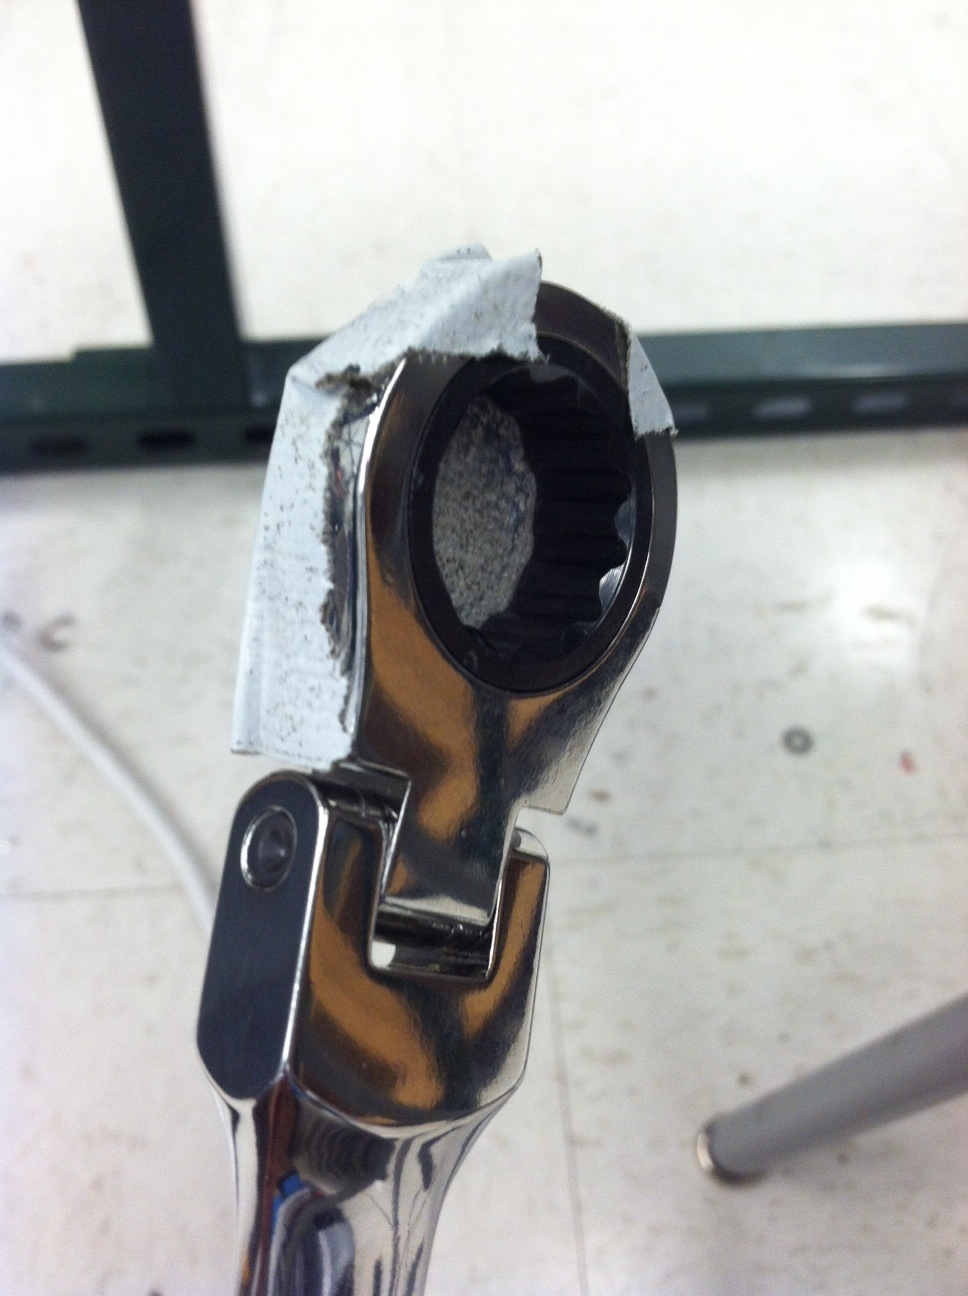
\includegraphics[width = 2.75in]{photoAlign1.JPG}
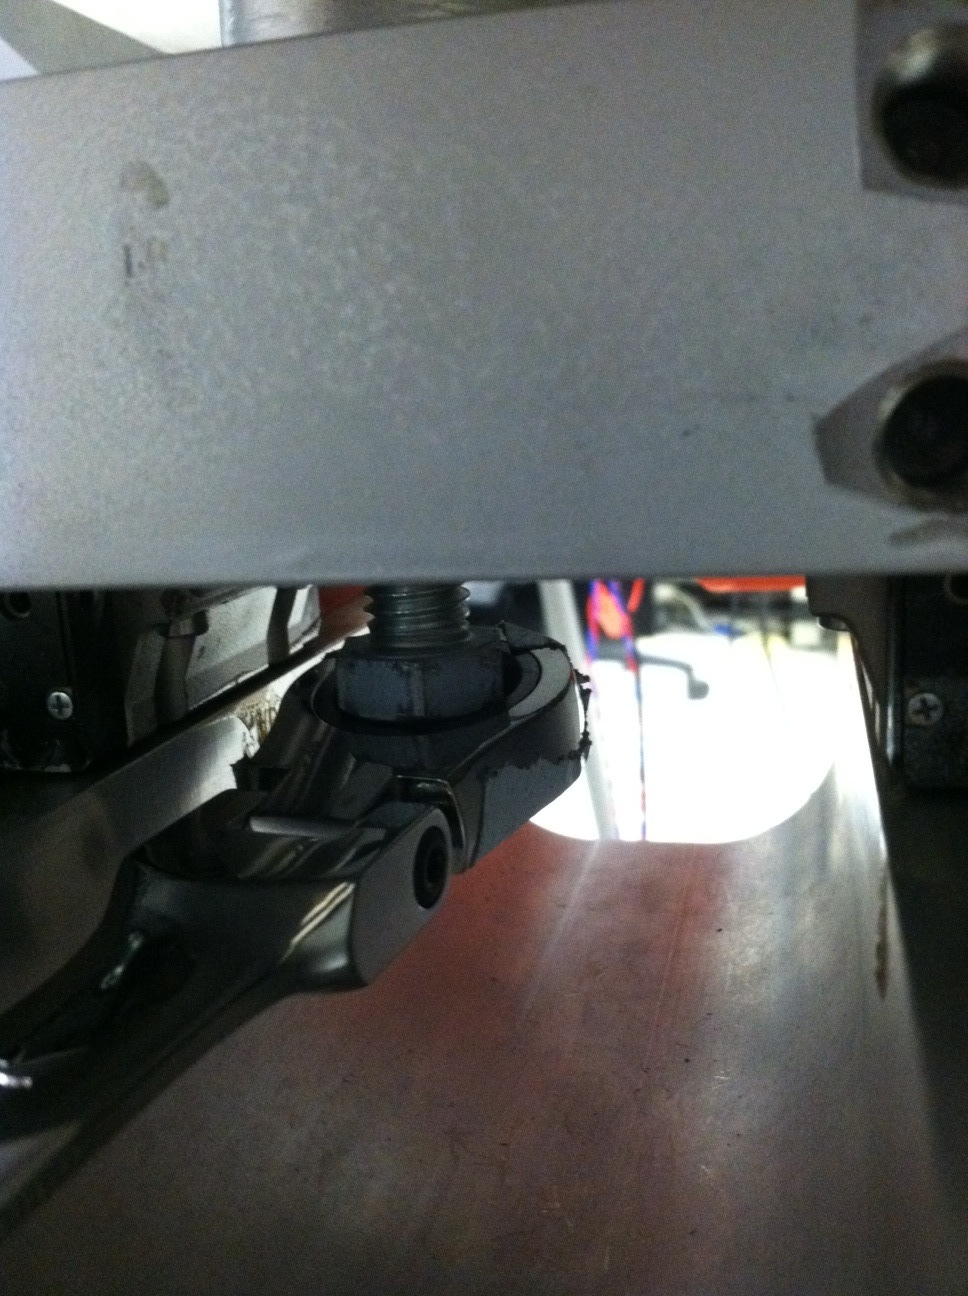
\includegraphics[width = 2.75in]{photoAlignTwo.JPG}
\caption{}  
\label{figAlign}
\end{center}
\end{figure}

\begin{figure}[h]
\begin{center}
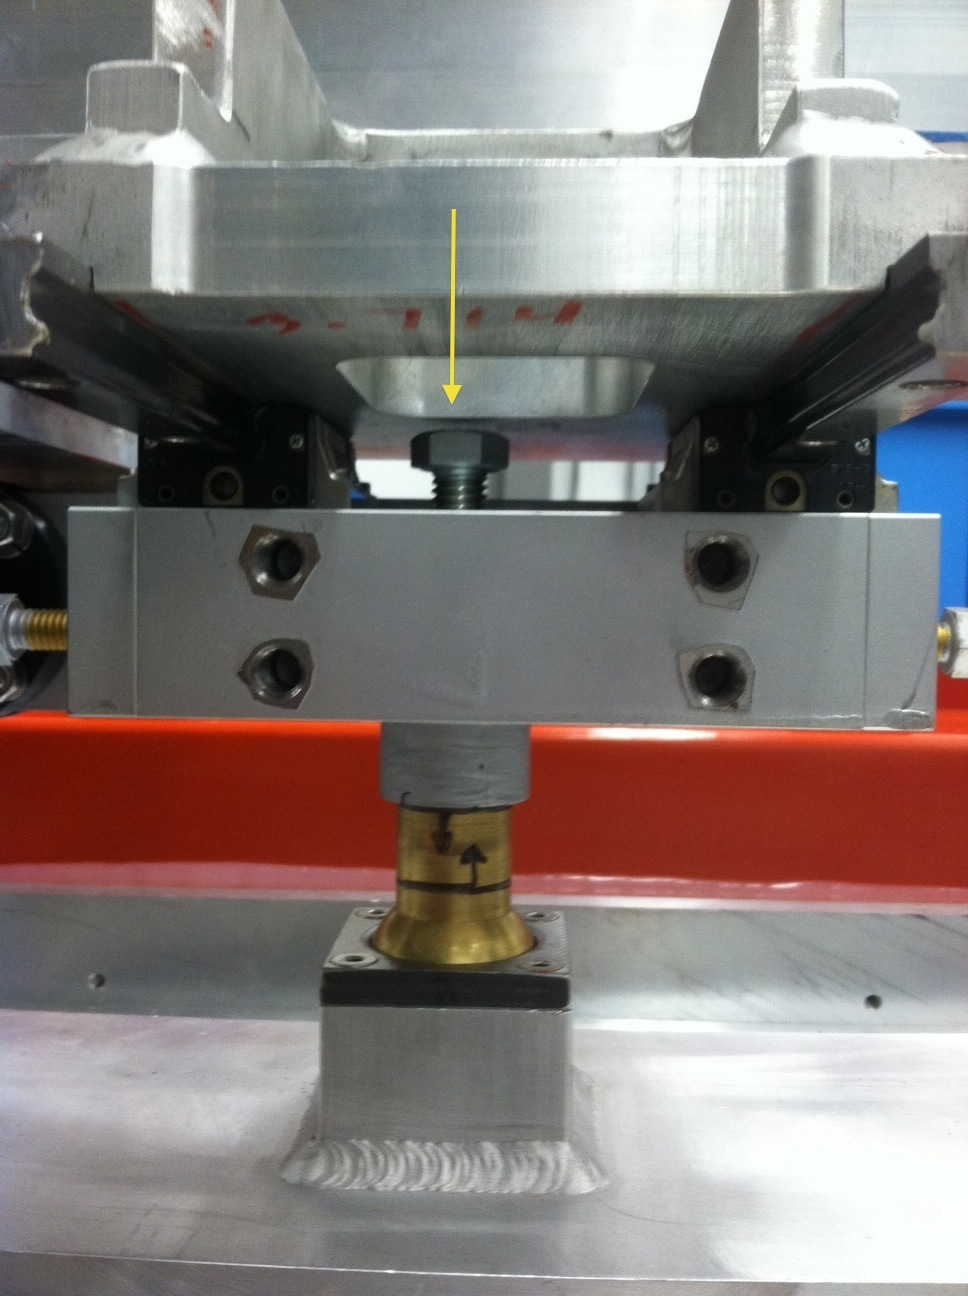
\includegraphics[width = 2.75in]{screwWarning.JPG}
\caption{}  
\label{figAlign2}
\end{center}
\end{figure}


\section{Troubleshooting}

\subsection{Problem with the motor drivers}
The LEDs on each of the three motor drivers in the electronics box will be solid green if everything is ok.
The fact that they are solid green means that they are powered, configured properly, and that they are sitting idle.  
If there is a problem in the configuration or hardware, it will likely show up here.
\begin{itemize}
 	\item Blinking red:  Check to make sure that all three motor cables are properly connected.  
		A motor will be red if it can't find the hardware.  Otherwise, the motor driver may need to be reconfigured.
	\item Blinking green:  This means that the motor is powered and configured, but not sitting idle.  You may have to reload the arduino sketch.  If that doesn't work, reload the motor 		configuration again.
	\item For other combination of blinks and colors, see the LED codes listed in Fig. \ref{ledCodes}
\end{itemize}

\begin{figure}[h]
\begin{center}
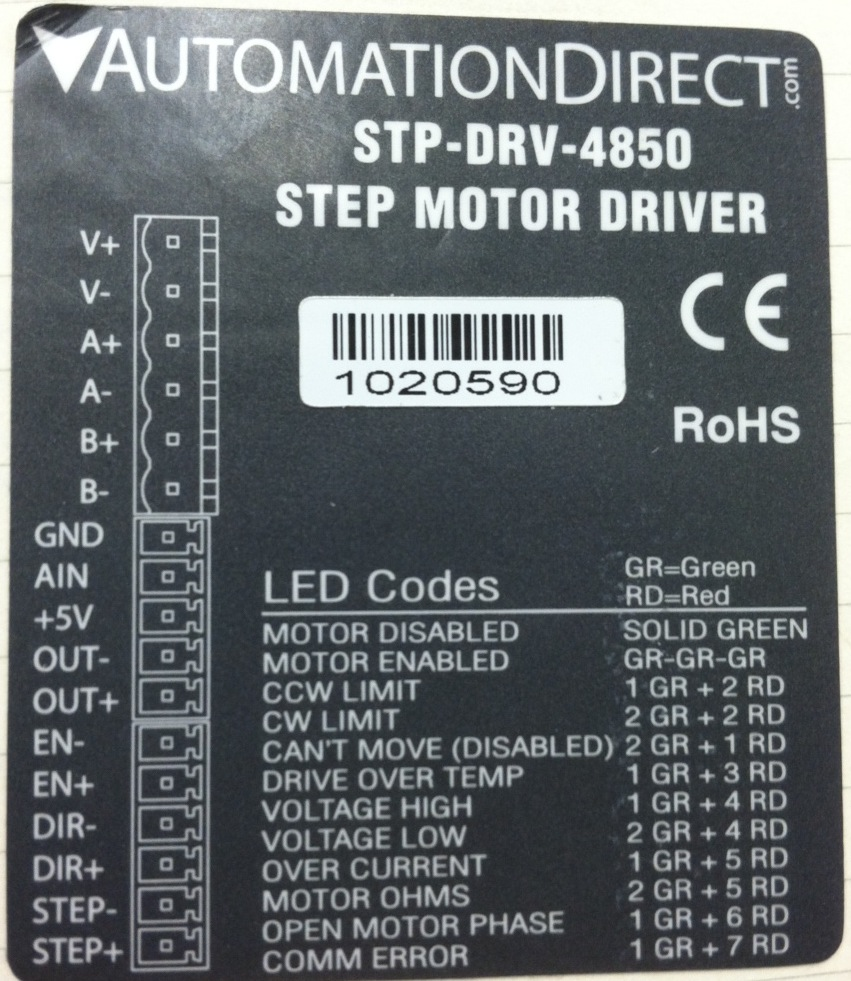
\includegraphics[width = 2.2in]{photoLedCodes.JPG}
\caption{Motor driver LED codes.}  
\label{ledCodes}
\end{center}
\end{figure}

\subsection{Problems with the stored camera information}
If power is lost at any time, it might be the case that one of the following files gets deleted: position.txt, range.txt, alignment.txt. 
The information in each of these files is loaded into memory when the program is started.
The arduino sketch needs to know the camera location to move.
This is because there are limits set and calculated each time you request the telescope to move.
This system is based on these text files - and you don't hit the limits!
Each of these files sits inside a directory on the arduino SD care: /mnt/sda1\\[15pt]
If position.txt, or range.txt is missing:
\begin{enumerate}
\item[1.] Go into alignment mode if not there already and find the camera range (see "Setting Range" above).
\item[2.] Hit GETALGN to request the stored alignment position.
\item[3.] Manually move the camera to the alignment position.
\item[4.] Go back to the normal operation mode.
\end{enumerate}
If alignment.txt is missing realign the camera. Sorry :/. (This should never happen)

\subsection{Problems with a Yun}
See Sec. \ref{secYun} for more details.
If the $\mu$SD card is ok, you should be able to simply put the card into a new Yun and roll.

\section{Replacing a Yun with a new Yun that isn't configured}
\label{secYun}
\begin{enumerate}
\item Plug Yun into laptop via micro usb.
\item Look for the Yun's wifi network. If it doesn't appear, hold the wlan reset button until it blinks.
\item If the Yun's wifi network still doesn't appear try plugging the Yun ethernet into your LAN and connect to the Yun or Linino's network. Continue below as appropriate.\\
\item Are you using a Linino or Arduino?
        	\begin{itemize} 
		\item {\textbf{Linino:}} Open a browser and go to 192.168.240.1 and login to the Linino web UI. The default password is 'doghunter'.
		\item {\textbf{Arduino:}} Open a browser and go to arduino.local and login to the Arduino web UI. The default password is 'arduino' or 'arduino1'.
	\end{itemize}
\item \textbf{Continue Here:} Click on the advanced configuration at the top of the page.
\item Go to the network tab and click edit on the WAN panel.
\item Switch the network protocol to static ip.
\item Enter LAN ip reserved for the Yun along with the gateway ip and network mask. Hit save.
\item If required go to the wifi panel and disable the wifi.

\item If desired, set up the LAN to forward incoming requests from some port to the Yun ip.\\
\item \textbf{Loading the sketch:} If the previous Yun's sd card is still accessible just put it into the new Yun. Otherwise get a fresh sd card and download the Yun sd expander sketch (Google it).
\item If necessary find the Yun's ip address on the LAN and go that ip in your web browser. Then open up the Arduino IDE and select that same ip as the port. Upload the sd expander (and or the motion control sketch) if necessary.

\item After loading from the Arduino IDE you should see all the green lights on for the three motor drivers (not flashing).  
The motor drivers are located in the electronics box, see the wiring diagram below.

\item {\textbf{If you are using a Linino:}}  If the Ardiuno is a Linino you may have to create a symbolic link for the OS to know where to look for the website.  
After these steps you should be able to load the webpage via [ArduinoIP] / [sd].  
If you can already connect, all is good already.
	\begin{itemize}
		\item ssh -Y root@[IP address]
		\item cd /www/
		\item ln -s /mnt/sda1/sd
	\end{itemize}
	
\item Note that with a fresh install you will need to physically create all the text files discussed above (position.txt, range.txt, alignment.txt).
	The procedure to do this is detailed in previous sections.
\end{enumerate}


\section{Removing the Inner Camera Structure}
We show here a step-by-step of removing the inner camera structure.  
Note that a lifting crane is absolutely necessary, the inner structure is very heavy.
We used a purple strap connected to an overhead crane that you will see in the pictures.

\begin{enumerate}
\item Ratchet down bottom screws (screws pushing up on the holding pins)
\item Move camera all the way forward
\item Allen wrench off the top piece holding in the pin.  See Figure \ref{figRemove1}.
\item Jiggle to get the ball to disconnect
\item Pop top ball joint out.  Now the top tilts forward.  See Figure \ref{figRemove2}.
\item Pull it up straight.
\item Pop out one of the two bottom pins (take it out 'leg-by-leg'). 
\item Lift manually out the other side pin
\item Don't drop it.  Seriously.
\end{enumerate}

\begin{figure}[h]
\begin{center}
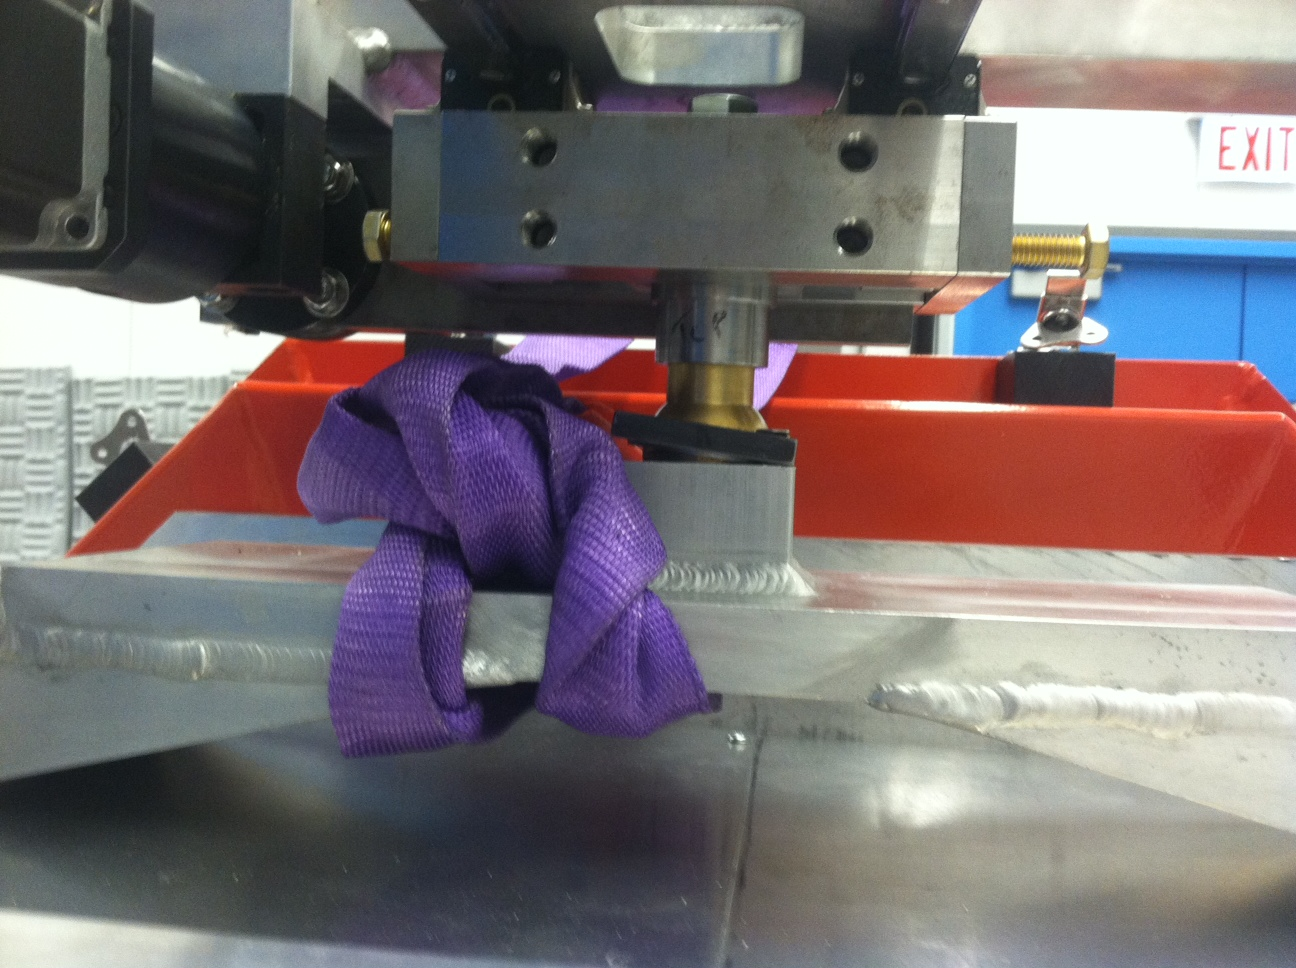
\includegraphics[width = 3in]{photo_2.png}
\end{center}
\caption{}  
\label{figRemove1}
\end{figure}


\begin{figure}[h]
\begin{center}
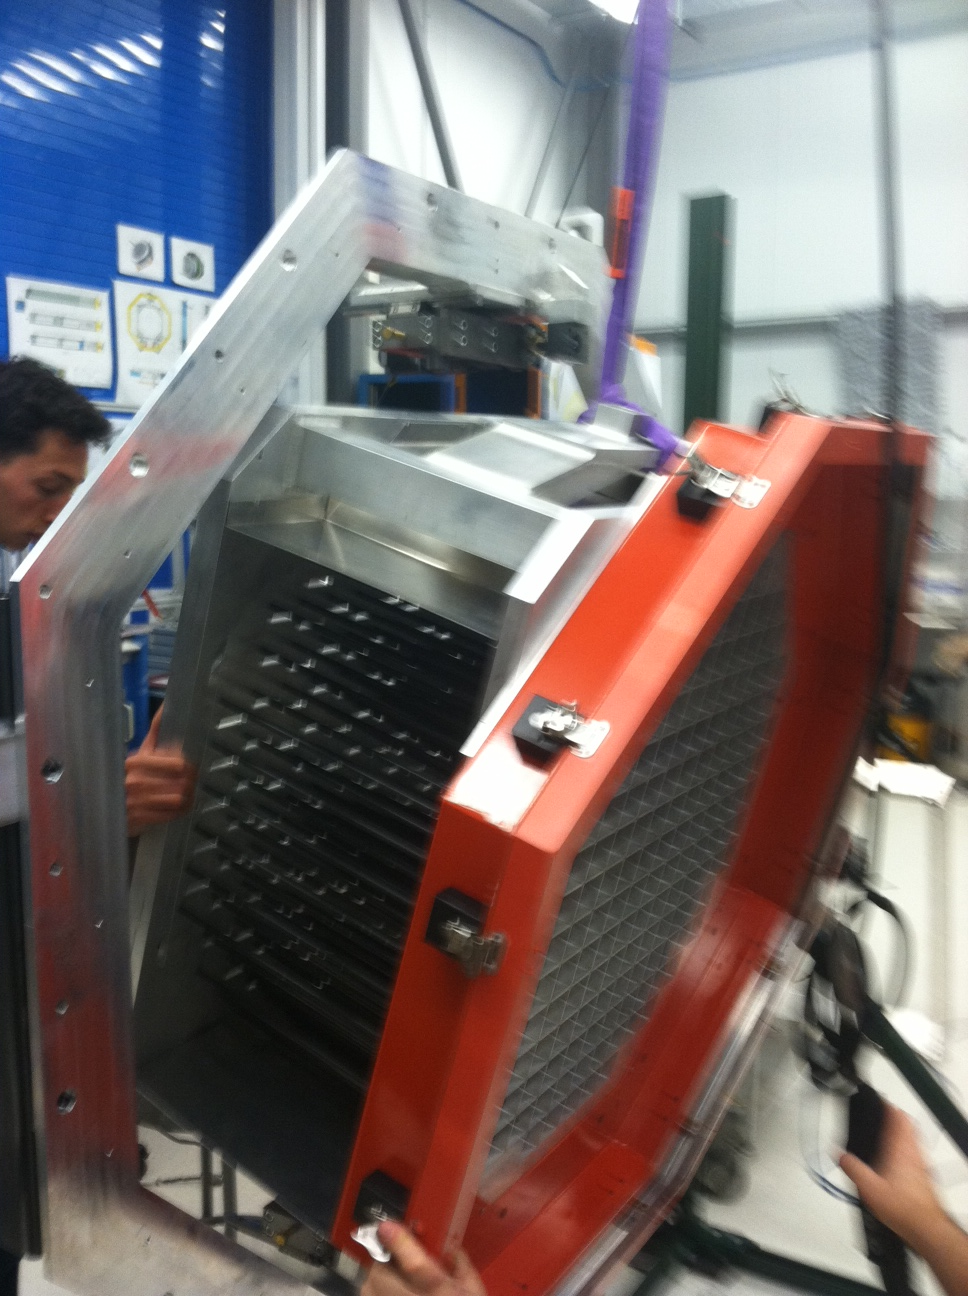
\includegraphics[width = 3in]{photo_3.png}
\end{center}
\caption{}  
\label{figRemove2}
\end{figure}


\section{Mounting the Inner Camera Structure}
We show here a step-by-step to mount the inner camera structure.  
Note that a lifting crane is absolutely necessary, the inner structure is very heavy.
We used a purple strap connected to an overhead crane that you will see in the pictures.

\begin{enumerate}
\item Move bottom motors all the way forward, the top motor all the way back.
\item Make sure the screws for the holding ball pins are ratcheted all the way down.
\item Put one lower ball joint in place
\item Bring the whole inner structure down to sink that one in
\item Pivot to put the other lower pin in
\item Now lower the inner structure all the way down until it is resting (you need clearance for the top pin)
\item Put the top ball pin in all the way and hold it there (you may have to ratched the screw up all the way)
\item Pivot the camera structure to put the ball into place 
\item Attach the ball pin holding frame with 1/8 inch allen
\item Ratchet up the bottom two nuts
\end{enumerate}





\section{Fan Assembly Details}

The camera cooling system consists of two banks of 4 fans blowing through a water cooled radiator.
Each fan is an ebm-pabst model DV 6224 and the power is supplied by an Acopian power supply.
The fan banks run at a nominal voltage of 24V and draws 7A.
Figure \ref{fanPic} shows the terminal to connect the fan bank wires properly.
Since the camera isn't fully populated, we have manufactured baffles to force the air through the active area. 
Figure \ref{bafflePic} shows the optimal baffle orientation.

\begin{figure}[h]
\begin{center}
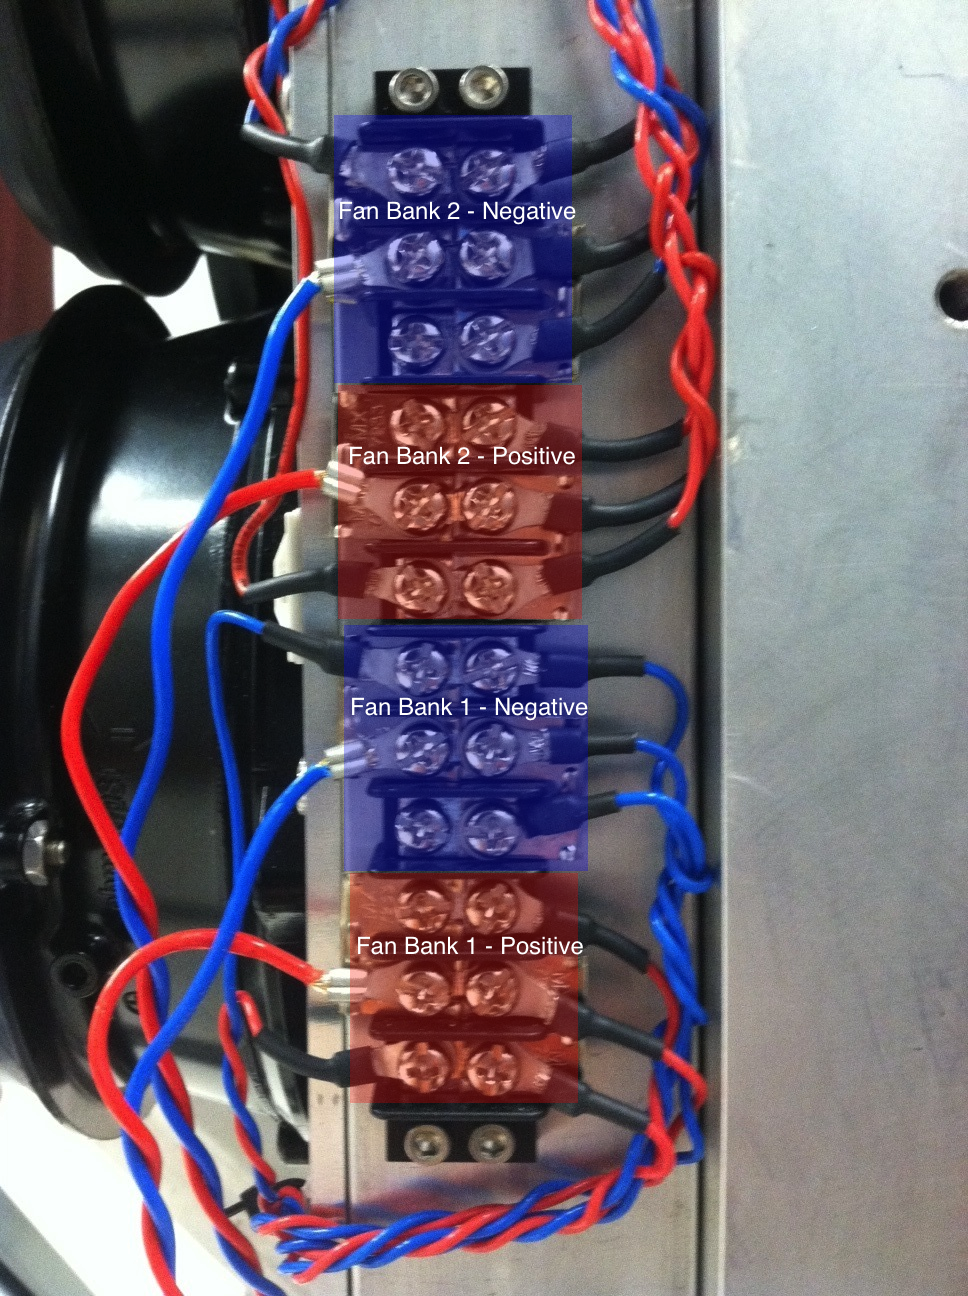
\includegraphics[width = 4in]{fanWiring.jpg}
\caption{Terminal block for fan assembly wiring.}  
\label{fanPic}
\end{center}
\end{figure}

\begin{figure}[h]
\begin{center}
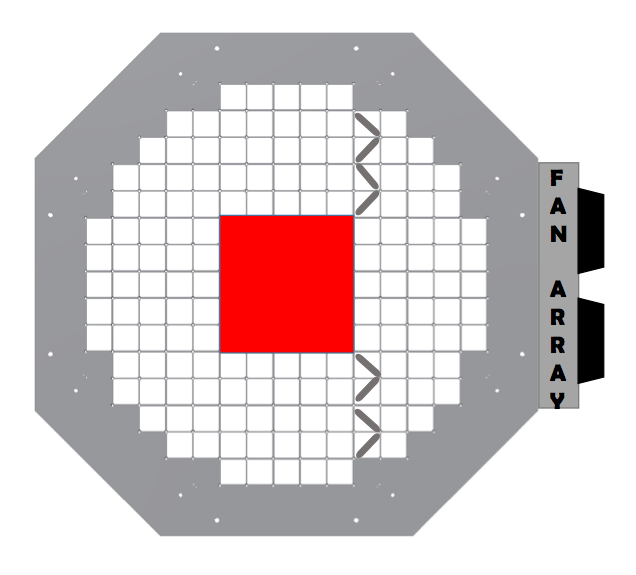
\includegraphics[width = 2.5in]{baffles.png}
\caption{Air baffle orientation.}  
\label{bafflePic}
\end{center}
\end{figure}



\newpage
\section{Tools in the Telescope Kit}

All the tools needed to drive each screw or bolt on the camera should be included in the camera toolbox. 
Additionally, there are spares for all the major components and connectors.
Have a look there first if you need something.
Here is what should be in there:

\begin{itemize}
	\item 3/4 inch flexible ratchet wrench with tape -- ball joint vertical centering screws for alignment
	\item 9/16 inch flexible ratchet wrench with tape -- ball joint horizontal centering screws for alignment
	\item 5/16 inch allen -- bolts for ball joint mount
	\item 7/32 inch allen -- Screw assembly bolts
	\item 2.5 mm allen -- slides
	\item 7/16 inch wrench (2x) -- screw flange bolts to connect screw to frame
	\item 3/16 inch wrench (2x) -- small wrenches for electronics box nuts
	\item 1/16 inch allen -- set screws for motor pins
	\item Phillips or flathead screwdriver -- everything else
	\item Spare $\mu$SD card
	\item Spare stepper motor driver + wiring terminals
	\item Spare stepper motor
	\item Touch-up paint and grease
	\item Spare electronics box pars (switch, ethernet mount, etc.)
	\item Spare horizontal alignment screw - allen head, extra long
\end{itemize}


\section{Electronics Box Wiring Diagram}
\begin{figure}[h]
\begin{center}
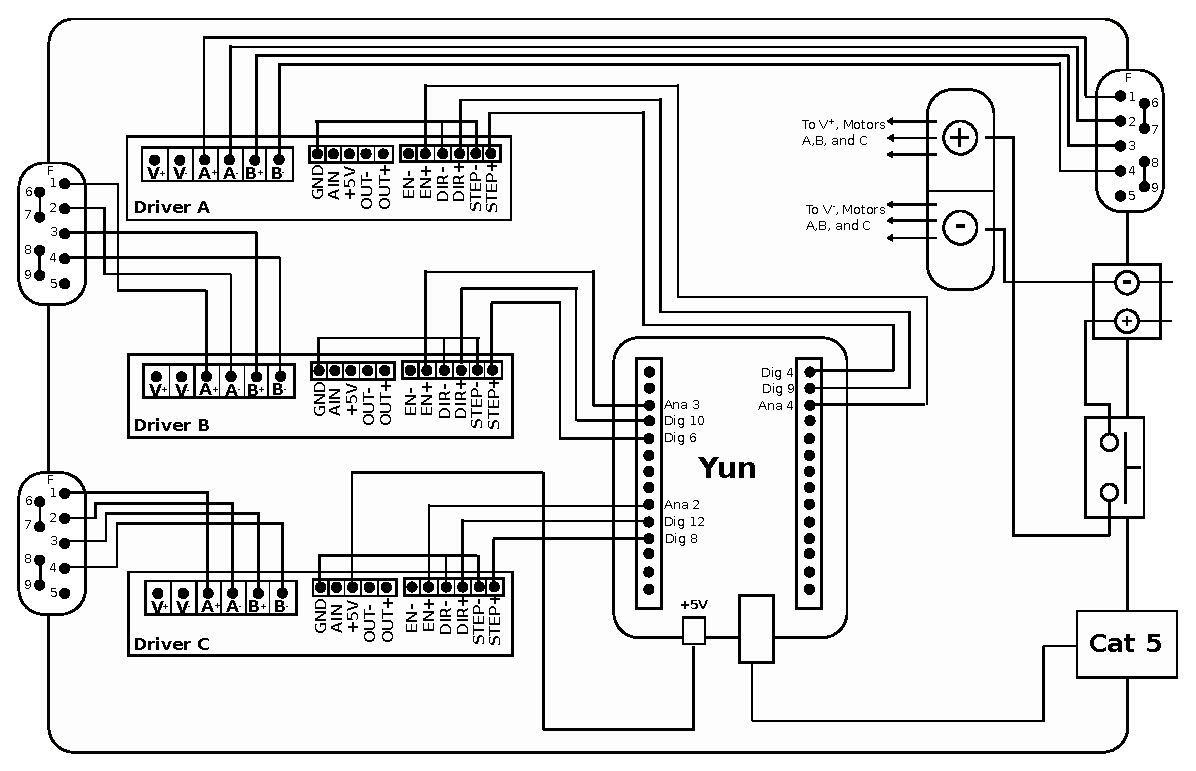
\includegraphics[width = 5.5in]{wiringDrawingUpdate.eps}
\caption{Wiring diagram for the electrical control box.}  
\label{fd2}
\end{center}
\end{figure}


\end{document}
